\documentclass[12pt, tikz]{standalone}
\usetikzlibrary{arrows.meta, calc, intersections, quotes}
\tikzset{
  dim line distance/.initial=.2cm,
  dim line style/.style={<->},
  dim line delim/.style={-, shorten <=2\pgflinewidth, shorten >=-7\pgflinewidth},
  dim line text/.style={midway, auto=left, font=\footnotesize},
  pics/dim line/.style args={#1--#2}{code={
    \draw[dim line style]
      ($(#1)!\pgfkeysvalueof{/tikz/dim line distance}!90:(#2)$) coordinate (@1)
      to node[dim line text,style/.expand once=\tikzpictextoptions]{$\tikzpictext$}
      ($(#2)!\pgfkeysvalueof{/tikz/dim line distance}!-90:(#1)$)coordinate (@2);
    \draw[dim line delim] (#1) to (@1);
    \draw[dim line delim] (#2) to (@2);}}}
\begin{document}
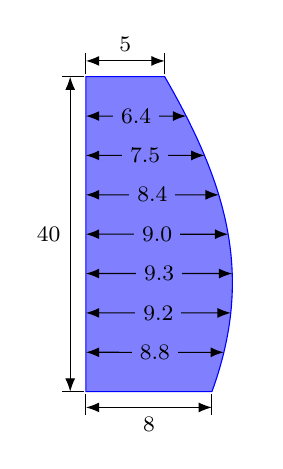
\begin{tikzpicture}[> = Latex, x = .2cm, y = 0.1cm]

\draw[draw=blue,fill=blue!50, name path=area]
                        (0, 0) coordinate (bl)
                  -- (right:8) coordinate (br)
  to[out=70, in=-60] +(-3, 40) coordinate (tr)
                            -| coordinate (tl) cycle;

\pic ["40"] {dim line=bl--tl}
 pic [ "8"] {dim line=br--bl}
 pic [ "5"] {dim line=tl--tr};

\foreach \level in {1, ..., 7} {
  \path[overlay, help lines, name path=hor\level]
    (10pt, \level/8*40) -- +(right:10);
  \draw[name intersections={of=area and hor\level, by=is-\level},
    <->, nodes={fill=blue!50, node font=\footnotesize},
    /pgf/number format/.cd, fixed zerofill, precision=1]
    let \p 0 = ($(is-\level) - (0,0)$),
        \p B = ($(br)        - (bl) $), % redundant
        \n 0 = {scalar(\x0/\x B*8)} in  % scalar removes units
    (0, \level/8*40) -- node {$\pgfmathprintnumber{\n0}$} (is-\level);
}
\end{tikzpicture}
\end{document}